\documentclass[tikz,border=5mm]{standalone}
\usepackage{tikz}
\usetikzlibrary{arrows.meta, positioning, shapes.geometric, calc, backgrounds, fit, matrix, patterns, decorations.pathmorphing, shadows}

% --- COLOR DEFINITIONS ---
\definecolor{Garnet}{HTML}{73000A}
\definecolor{CSecondaryRed}{HTML}{CC2E40}
\definecolor{CBlue}{HTML}{466A9F}
\definecolor{CDark}{HTML}{1F414D}
\definecolor{COlive}{HTML}{65780B}
\definecolor{CLime}{HTML}{CED318}
\definecolor{CGold}{HTML}{A49137}
\definecolor{CGrayLight}{HTML}{E5E5E5}
\definecolor{CGrayDark}{HTML}{555555}
\definecolor{CWhite}{HTML}{FFFFFF}
\definecolor{CBlack}{HTML}{000000}

\begin{document}

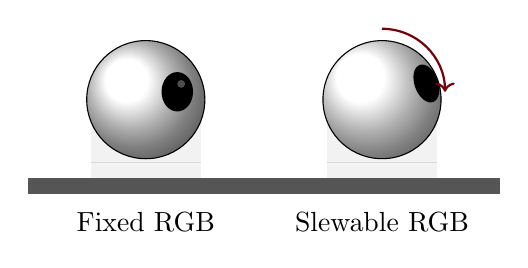
\begin{tikzpicture}
    \def\flircam{
        % Base
        \fill[CWhite!90!gray] (-0.7, 0) rectangle (0.7, 1.0);
        \draw[gray!30] (-0.7, 0.2) -- (0.7, 0.2);
        \node[font=\tiny\sffamily, text=CDark] at (0, 0.5) {FLIR};
        
        % Rotating Head (Dome)
        \shadedraw[ball color=CWhite] (0, 1.0) circle (0.75);
        \fill[black] (0.4, 1.1) ellipse (0.2 and 0.25); % Lens
        \fill[white, opacity=0.3] (0.45, 1.2) circle (0.05); % Glint
    }

    % Tripod Top Plate
    \fill[CGrayDark] (-3, -0.2) rectangle (3, 0);
    
    % Cam 1
    \begin{scope}[shift={(-1.5, 0)}]
        \flircam
        \node[below=0.3cm] {Fixed RGB};
    \end{scope}

    % Cam 2
    \begin{scope}[shift={(1.5, 0)}]
        % Base
        \fill[CWhite!90!gray] (-0.7, 0) rectangle (0.7, 1.0);
        \draw[gray!30] (-0.7, 0.2) -- (0.7, 0.2);
        \node[font=\tiny\sffamily, text=CDark] at (0, 0.5) {FLIR};
        
        % Rotating Head (Dome) - Tilted
        \begin{scope}[rotate around={20:(0, 1.0)}]
            \shadedraw[ball color=CWhite] (0, 1.0) circle (0.75);
            \fill[black] (0.6, 1.0) ellipse (0.15 and 0.25); % Lens side view
        \end{scope}
        
        % Motion arrows
        \draw[->, thick, Garnet] (0, 1.9) arc (90:0:0.8);
        
        \node[below=0.3cm] {Slewable RGB};
    \end{scope}

\end{tikzpicture}

\end{document}
